\subsection{Eigenvector Correspondence}
\label{sec:app_exp_corr}

In this section, we leverage the idea of eigenvector matricization (\definitionref{def:matricization}) and analyze the validity of the decoupling conjecture using a matrix which we defined as the eigenvector corresponding matrix. First let us recall the definition of eigenvector matricization

\paragraph{\definitionref{def:matricization}} \emph{Consider a layer with input dimension $n$ and output dimension $m$. For an eigenvector $\vh\in\R^{mn}$ of its layer-wise Hessian, the matricized form of $\vh$ is $\Mat(\vh)\in\R^{m\times n}$ where $\Mat(\vh)_{i,j} = \vh_{(i-1)m+j}$.}
\vspace{1em}

Suppose the $i$-th eigenvector for $\E[\vx\vx^\T]$ is $\vv_i$ and the $j$-th eigenvector for $\E[\mM]$ is $\vu_j$. Then the Kronecker product $\E[\mM]\otimes \E[\vx\vx^\T]$ has an eigenvector $\vu_j\otimes \vv_i$. Therefore if the decoupling conjecture is true, one would expect that the top eigenvector of the layer-wise Hessian have a clear correspondence with the top eigenvectors of its two components. Note that $\vu\otimes\vv$ is just the flattened matrix $\vu\vv^\T$.

More concretely, to demonstrate the correspondence between the eigenvectors of the layerwise hessian and the eigenvectors of matrix $\E[\mM]$ and $\E[\vx\vx^\T]$, we introduce ``eigenvector correspondence matrices'' as shown in \figureref{fig:Corr_fc}.
\begin{definition}[Eigenvector Correspondence Matrices]
For layer-wise Hessian matrix $\mH\in\R^{mn\times mn}$ with eigenvectors $\vh_1, \cdots, \vh_{mn}$, and its corresponding auto-correlation matrix $\E[\vx\vx^\T]\in\R^{n\times n}$ with eigenvectors $\vv_1, \cdots, \vv_n$. The correspondence between $\vv_i$ and $\vh_j$ can be defined as \begin{equation}
    \Corr(\vv_i,\vh_j) := \|\Mat(\vh_j)\vv_i\|^2.
\end{equation}
For the output Hessian matrix $\E[\mM]\in\R^{m\times m}$ with eigenvectors $\vu_1, \cdots, \vu_m$, we can likewise define correspondence between $\vv_i$ and $\vh_j$ as
\begin{equation}
    \Corr(\vu_i,\vh_j) := \|\Mat(\vh_j)^\T\vu_i\|^2
\end{equation}
We may then define the eigenvector correspondence matrix between $\mH$ and $\E[\vx\vx^\T]$ as a $n\times mn$ matrix whose $i,j$-th entry is $\Corr(\vv_i,\vh_j)$, and the eigenvector correspondence matrix between $\mH$ and $\E[\mM]$ as a $m\times mn$ matrix whose $i,j$-th entry is $\Corr(\vu_i,\vh_j)$.
\label{def:corr_mat}
\end{definition}

Intuitively, if the $i,j$-th entry of the corresponding matrix is close to 1, then the eigenvector $\vh_j$ is likely to be the Kronecker product of $\vv_i$ (or $\vu_i$) with some vector. Note that if the decoupling conjecture holds absolutely, every eigenvector of the layer-wise Hessian (column of the correspondence matrices) should have a perfect correlation of 1 with exactly one of $\vv_i$ and one of $\vu_i$.
In \figureref{fig:Corr_fc} we can see that the correspondence matrices for the true layer-wise Hessian approximately satisfies this property for top eigenvectors. The similarity between the correspondence patterns for the true and approximated Hessian also verifies the validity of the Kronecker approximation for dominating eigenspace.

% \begin{figure}[th]
%     \centering
%     \subfigure[\small{True Hessian with $\E[\vx\vx^\T].$}]{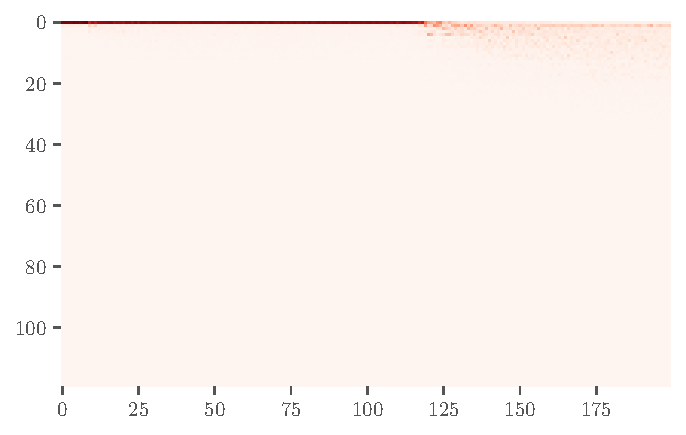
\includegraphics[width=0.45\textwidth]{Figures/Correspondence/LeNet5_fixlr0.01/xxT_Trueest_real_corr_expand_t200_CIFAR10_Exp1_LeNet5_fixlr0.01R2_E-1_fc1.pdf}}
%     \subfigure[\small{True Hessian with $\E[\mM^\T].$}]{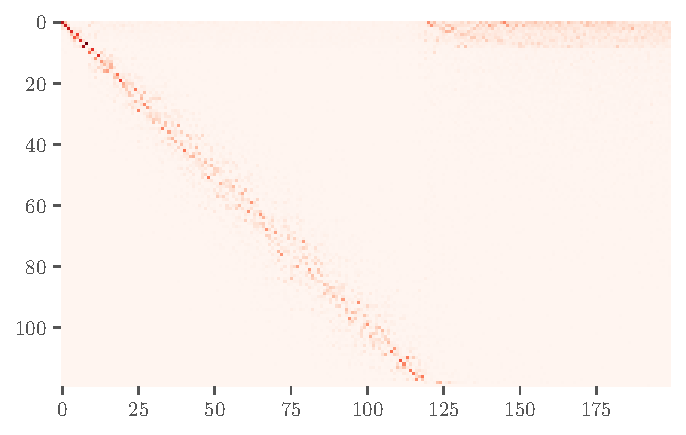
\includegraphics[width=0.45\textwidth]{Figures/Correspondence/LeNet5_fixlr0.01/UTAU_Trueest_real_corr_expand_t200_CIFAR10_Exp1_LeNet5_fixlr0.01R2_E-1_fc1.pdf}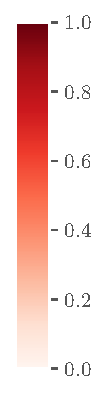
\includegraphics[width=0.06\textwidth]{Figures/Misc/colorbar.pdf}}
%     \\
%     \subfigure[\small{Approx Hessian with $\E[\vx\vx^\T].$}]{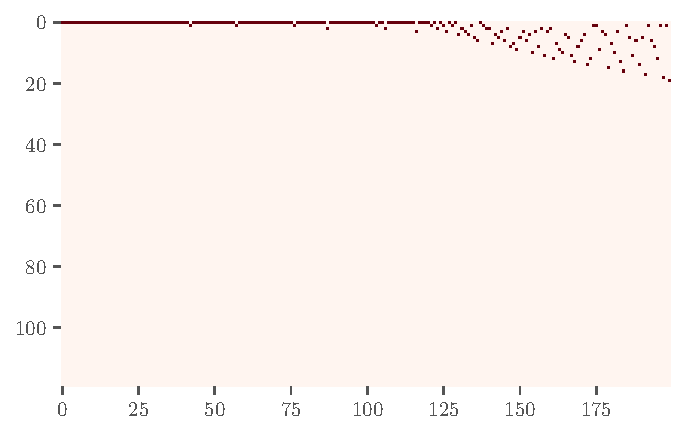
\includegraphics[width=0.45\textwidth]{Figures/Correspondence/LeNet5_fixlr0.01/xxT_Approxest_real_corr_expand_t200_CIFAR10_Exp1_LeNet5_fixlr0.01R2_E-1_fc1.pdf}}
%     \subfigure[\small{Approx Hessian with $\E[\mM^\T].$}]{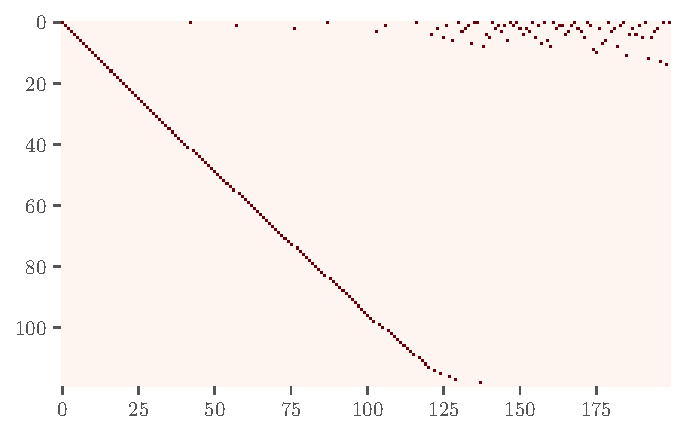
\includegraphics[width=0.45\textwidth]{Figures/Correspondence/LeNet5_fixlr0.01/UTAU_Approxest_real_corr_expand_t200_CIFAR10_Exp1_LeNet5_fixlr0.01R2_E-1_fc1.pdf}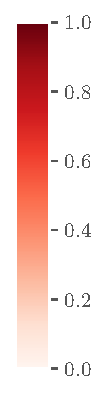
\includegraphics[width=0.06\textwidth]{Figures/Misc/colorbar.pdf}}
%     \caption{Heatmap of Eigenvector Correspondence Matrices for fc1:LeNet5, which has 120 output neurons. Here we take the top left corner of the eigenvector correspondence matrices. We can see that the top 120 eigenvectors of $\E[\mH]$, roughly corresponds to the top 120 eigenvectors of $\E[\mM]$ (as shown by the diagonal patter of (\emph{b})) and the first eigenvector of $\E[\vx\vx^\T]$ (as shown by the horizontal pattern of (\emph{a})). The similarity between the first row and the second row also shows the validity of the Kronecker approximation}
%     \label{fig:Corr_fc}
%     \vspace{-1em}
%     % \vspace{-4em}
% \end{figure}
In \figureref{fig:Corr_fc}, we show the heatmap of Eigenvector Correspondence Matrices for fc1:LeNet5, which has 120 output neurons. Here we take the top left corner of the eigenvector correspondence matrices. We can see that the top 120 eigenvectors of $\E[\mH]$, roughly corresponds to the top 120 eigenvectors of $\E[\mM]$ (as shown by the diagonal patter of (\emph{b})) and the first eigenvector of $\E[\vx\vx^\T]$ (as shown by the horizontal pattern of (\emph{a})). The similarity between the first row and the second row also shows the validity of the Kronecker approximation.
\label{sec:eigen_corr}
\begin{figure}[H]
    \centering
    \begin{subfigure}[t]{0.46\textwidth}
        \centering
        \captionsetup{justification=centering}
        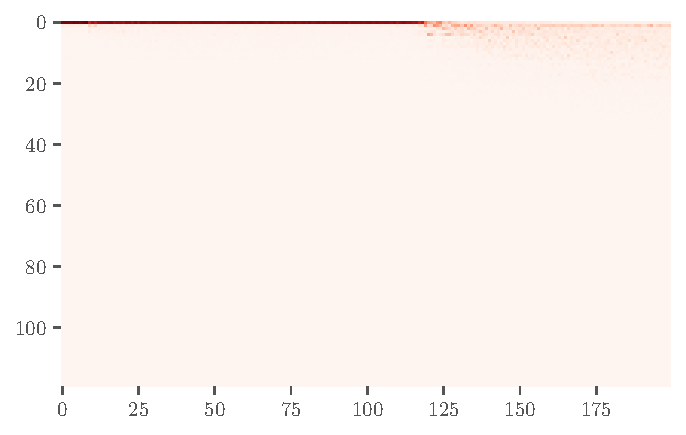
\includegraphics[width=0.9\textwidth]{Figures/Correspondence/LeNet5_fixlr0.01/xxT_Trueest_real_corr_expand_t200_CIFAR10_Exp1_LeNet5_fixlr0.01R2_E-1_fc1.pdf}
        \caption{True Hessian with $\E[\vx\vx^\T].$}
        \label{fig:Corr_xxT_True_fc}
    \end{subfigure}%
    \begin{subfigure}[t]{0.46\textwidth}
        \centering
        \captionsetup{justification=centering}
        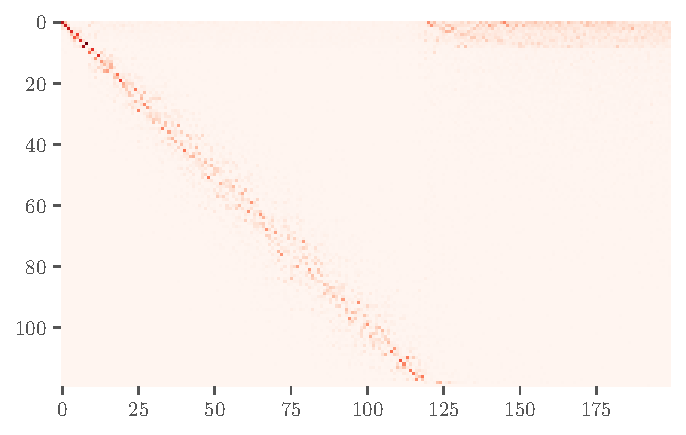
\includegraphics[width=0.9\textwidth]{Figures/Correspondence/LeNet5_fixlr0.01/UTAU_Trueest_real_corr_expand_t200_CIFAR10_Exp1_LeNet5_fixlr0.01R2_E-1_fc1.pdf}
        \caption{True Hessian with $\E[\mM].$}
        \label{fig:Corr_UTAU_True_fc}
    \end{subfigure}%
    \begin{subfigure}[t]{0.065\textwidth}
        \centering
        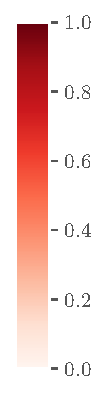
\includegraphics[width=\textwidth]{Figures/Misc/colorbar.pdf}
    \end{subfigure}
    \bigskip
\begin{subfigure}[t]{0.46\textwidth}
        \centering
        \captionsetup{justification=centering}
        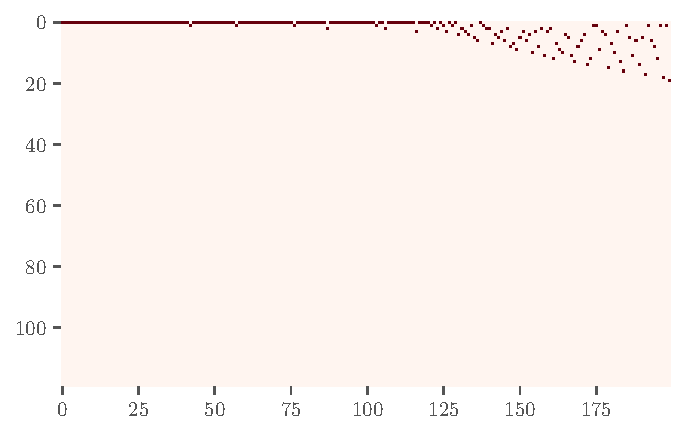
\includegraphics[width=0.9\textwidth]{Figures/Correspondence/LeNet5_fixlr0.01/xxT_Approxest_real_corr_expand_t200_CIFAR10_Exp1_LeNet5_fixlr0.01R2_E-1_fc1.pdf}
        \caption{Approximated Hessian with $\E[\vx\vx^\T].$}
        \label{fig:Corr_xxT_Approx_fc}
    \end{subfigure}%
    \begin{subfigure}[t]{0.46\textwidth}
        \centering
        \captionsetup{justification=centering}
        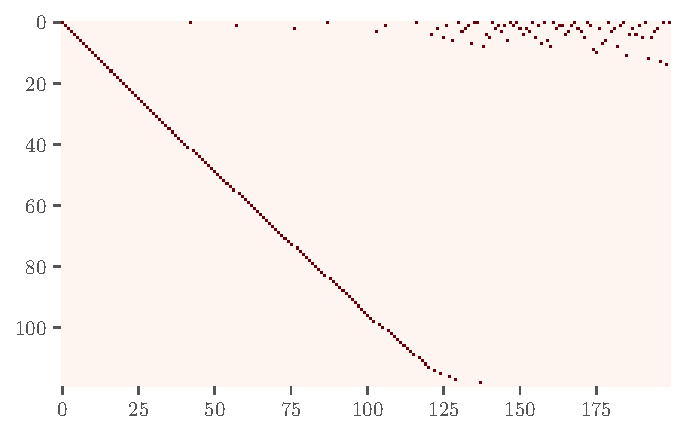
\includegraphics[width=0.9\textwidth]{Figures/Correspondence/LeNet5_fixlr0.01/UTAU_Approxest_real_corr_expand_t200_CIFAR10_Exp1_LeNet5_fixlr0.01R2_E-1_fc1.pdf}
        \caption{Approximated Hessian with $\E[\vx\vx^\T].$}
        \label{fig:Corr_UTAU_Approx_fc}
    \end{subfigure}%
    \begin{subfigure}[t]{0.065\textwidth}
        \centering
        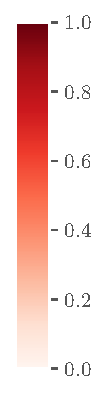
\includegraphics[width=\textwidth]{Figures/Misc/colorbar.pdf}
    \end{subfigure}
    \captionsetup{justification=centering}
    \caption{Heatmap of Eigenvector Correspondence Matrices for fc1:LeNet5.}
    \label{fig:Corr_fc}
\end{figure}

Here we present the correspondence matrix for fc2, conv1, and conv2 layer of LeNet5. The top eigenvectors for all layers shows a strong correlation with the first eigenvector of $\E[\vx\vx^\T]$ (which is approximately $\hE[\vx]$). For convolutional layers, since the computation of $\mM$ is not exact, the correspondence matrices with $\E[\mM]$ does not exhibit the diagonal pattern. For fc2:LeNet5 as in \figureref{fig:Corrfc22}, the diagonal pattern in (\emph{b}) and the strong correlation with $\E[\vx]$ stops at dimension 9. This fells into one of the ``failed cases'' as described in \sectionref{sec:appendix-failed-exp} case that the small eigenvalues of $\E[\rmM]$ are approaching $0$ faster than $\E[\vx\vx^\T]$. We will discuss this case in more detail in \sectionref{sec:appendix-failure}.


\begin{figure}[H]
    \centering
    \begin{subfigure}[t]{0.5\textwidth}
        \centering
        \captionsetup{justification=centering}
        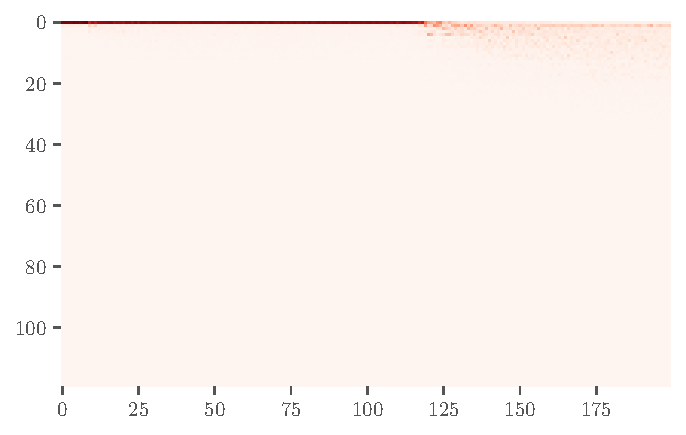
\includegraphics[width=\textwidth]{Figures/Correspondence/LeNet5_fixlr0.01/xxT_Trueest_real_corr_expand_t200_CIFAR10_Exp1_LeNet5_fixlr0.01R2_E-1_fc1.pdf}
        \caption{Correspondence with $\E[\vx\vx^T].$}
        \label{fig:Corr_xxT_True_fc1}
    \end{subfigure}%
    \begin{subfigure}[t]{0.5\textwidth}
        \centering
        \captionsetup{justification=centering}
        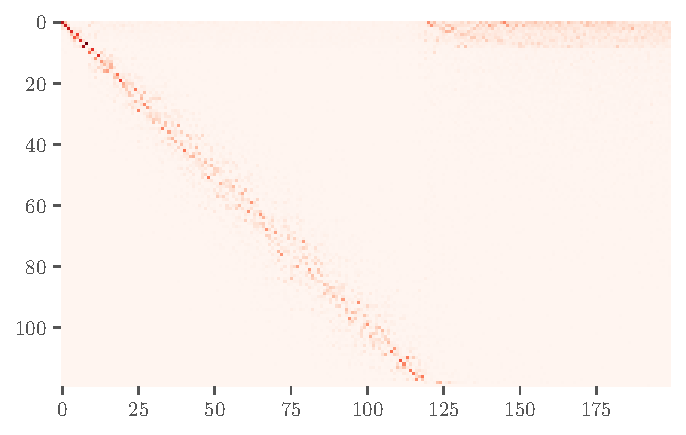
\includegraphics[width=\textwidth]{Figures/Correspondence/LeNet5_fixlr0.01/UTAU_Trueest_real_corr_expand_t200_CIFAR10_Exp1_LeNet5_fixlr0.01R2_E-1_fc1.pdf}
        \caption{Correspondence with $\E[\mM].$}
        \label{fig:Corr_UTAU_True_fc1}
    \end{subfigure}
    \caption{Eigenvector Correspondence for fc1:LeNet5. ($m$=120)}
    \label{fig:Corrfc11}
\end{figure}

\begin{figure}[H]
    \centering
    \begin{subfigure}[t]{0.5\textwidth}
        \centering
        \captionsetup{justification=centering}
        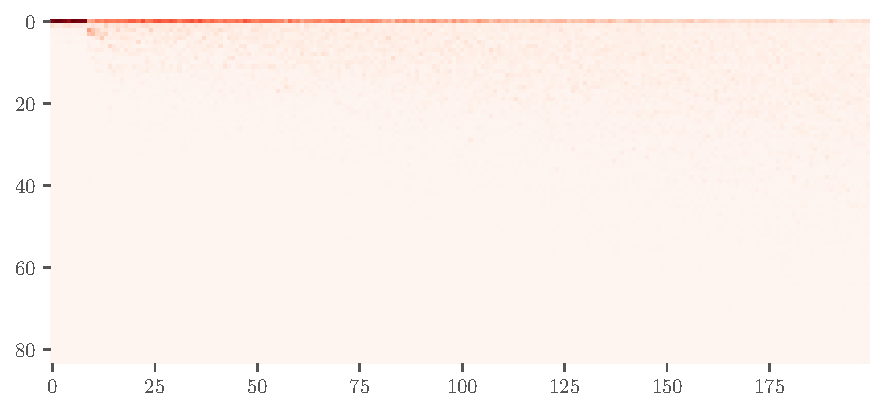
\includegraphics[width=\textwidth]{Figures/Correspondence/LeNet5_fixlr0.01/xxT_Trueest_real_corr_expand_t200_CIFAR10_Exp1_LeNet5_fixlr0.01R2_E-1_fc2.pdf}
        \caption{Correspondence with $\E[\vx\vx^T].$}
        \label{fig:Corr_xxT_True_fc2}
    \end{subfigure}%
    \begin{subfigure}[t]{0.5\textwidth}
        \centering
        \captionsetup{justification=centering}
        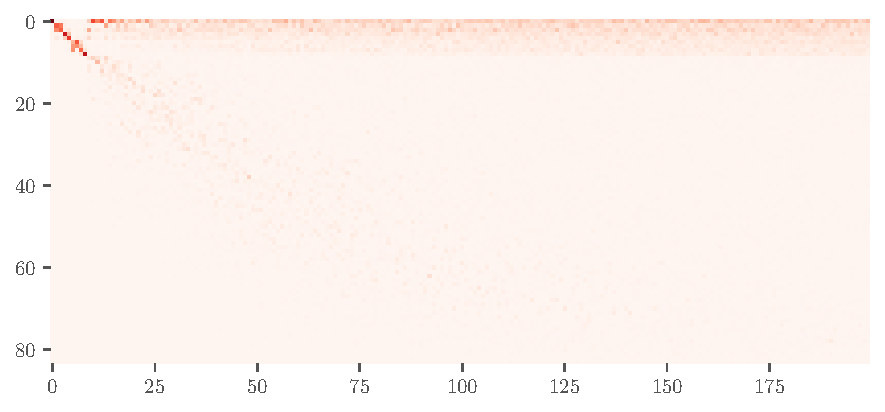
\includegraphics[width=\textwidth]{Figures/Correspondence/LeNet5_fixlr0.01/UTAU_Trueest_real_corr_expand_t200_CIFAR10_Exp1_LeNet5_fixlr0.01R2_E-1_fc2.pdf}
        \caption{Correspondence with $\E[\mM].$}
        \label{fig:Corr_UTAU_True_fc2}
    \end{subfigure}
    \caption{Eigenvector Correspondence for fc2:LeNet5. ($m$=84)}
    \label{fig:Corrfc22}
\end{figure}

\begin{figure}[H]
    \centering
    \begin{subfigure}[t]{0.5\textwidth}
        \centering
        \captionsetup{justification=centering}
        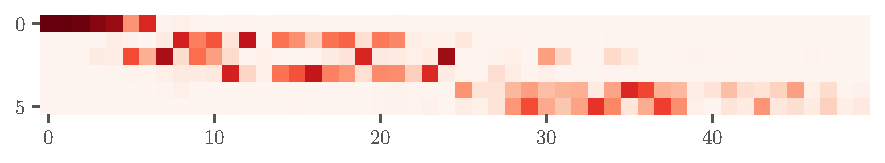
\includegraphics[width=\textwidth]{Figures/Correspondence/LeNet5_fixlr0.01/Conv/xxT_Trueest_real_corr_expand_t50_CIFAR10_Exp1_LeNet5_fixlr0.01_E-1_conv1.pdf}
        \caption{Correspondence with $\E[\vx\vx^T].$}
        \label{fig:Corr_xxT_True_conv1}
    \end{subfigure}%
    \begin{subfigure}[t]{0.5\textwidth}
        \centering
        \captionsetup{justification=centering}
        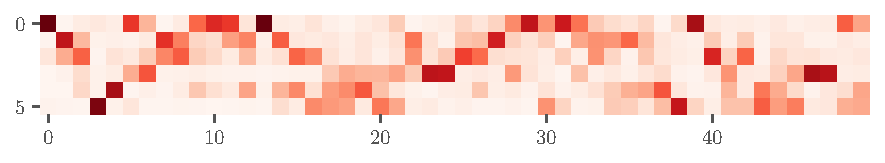
\includegraphics[width=\textwidth]{Figures/Correspondence/LeNet5_fixlr0.01/Conv/UTAU_Trueest_real_corr_expand_t50_CIFAR10_Exp1_LeNet5_fixlr0.01_E-1_conv1.pdf}
        \caption{Correspondence with $\E[\mM].$}
        \label{fig:Corr_UTAU_True_conv1}
    \end{subfigure}
    \caption{Eigenvector Correspondence for conv1:LeNet5. ($m$=6)}
    \label{fig:Corr_conv1}
\end{figure}

\begin{figure}[H]
    \centering
    \begin{subfigure}[t]{0.5\textwidth}
        \centering
        \captionsetup{justification=centering}
        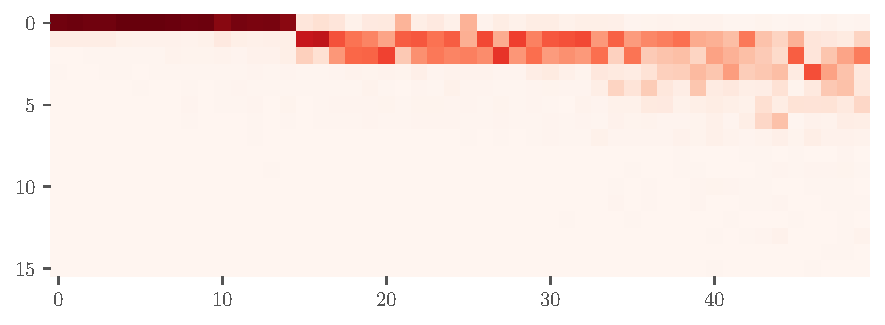
\includegraphics[width=\textwidth]{Figures/Correspondence/LeNet5_fixlr0.01/Conv/xxT_Trueest_real_corr_expand_t50_CIFAR10_Exp1_LeNet5_fixlr0.01_E-1_conv2.pdf}
        \caption{Correspondence with $\E[\vx\vx^T].$}
        \label{fig:Corr_xxT_True_conv2}
    \end{subfigure}%
    \begin{subfigure}[t]{0.5\textwidth}
        \centering
        \captionsetup{justification=centering}
        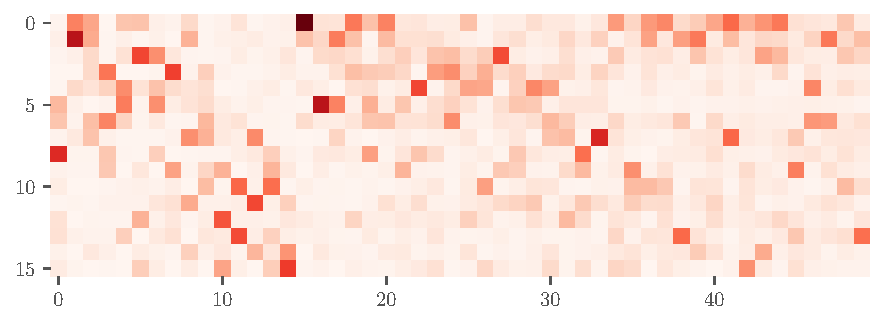
\includegraphics[width=\textwidth]{Figures/Correspondence/LeNet5_fixlr0.01/Conv/UTAU_Trueest_real_corr_expand_t50_CIFAR10_Exp1_LeNet5_fixlr0.01_E-1_conv2.pdf}
        \caption{Correspondence with $\E[\mM].$}
        \label{fig:Corr_UTAU_True_conv2}
    \end{subfigure}
    \caption{Eigenvector Correspondence for conv2:LeNet5. ($m$=16)}
    \label{fig:Corr_conv2}
\end{figure}


% \begin{figure}[H]
%     \centering
%     \subfigure[\small{Correspondence with $\E[\vx\vx^\T].$}]{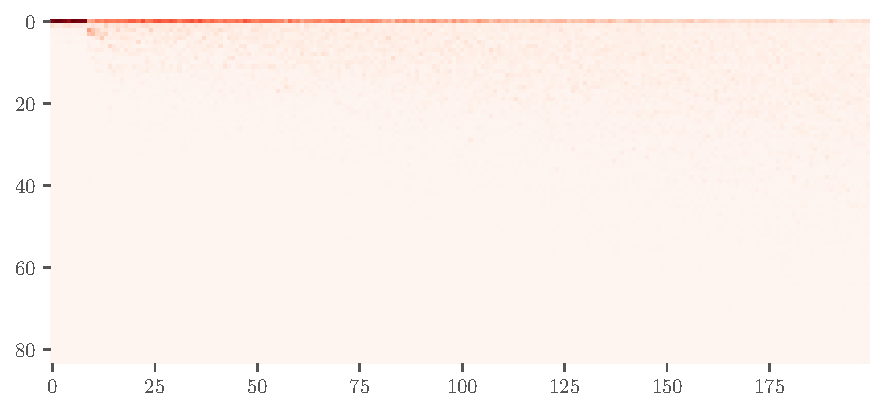
\includegraphics[width=0.45\textwidth]{Figures/Correspondence/LeNet5_fixlr0.01/xxT_Trueest_real_corr_expand_t200_CIFAR10_Exp1_LeNet5_fixlr0.01R2_E-1_fc2.pdf}}
%     \subfigure[\small{Correspondence with $\E[\mM].$}]{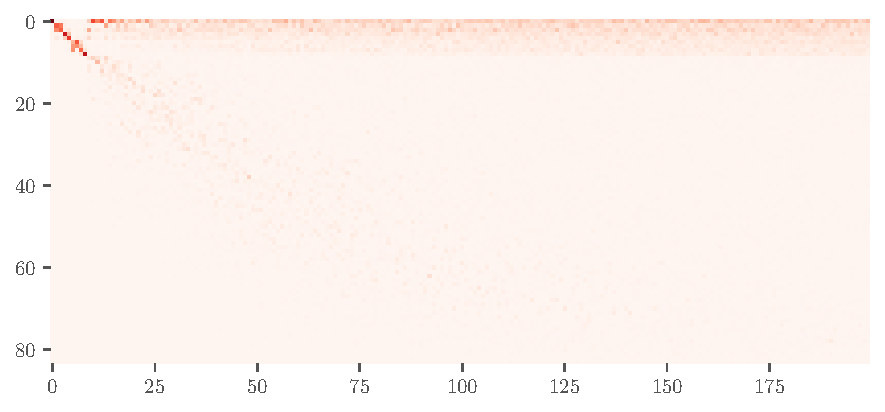
\includegraphics[width=0.45\textwidth]{Figures/Correspondence/LeNet5_fixlr0.01/UTAU_Trueest_real_corr_expand_t200_CIFAR10_Exp1_LeNet5_fixlr0.01R2_E-1_fc2.pdf}}
%     \caption{Eigenvector Correspondence for fc2:LeNet5. ($m$=84)}
%     \label{fig:Corr_fc2}
%     \vspace{-1em}
%     % \vspace{-4em}
% \end{figure}

% \begin{figure}[H]
%     \centering
%     \subfigure[\small{Correspondence with $\E[\vx\vx^\T].$}]{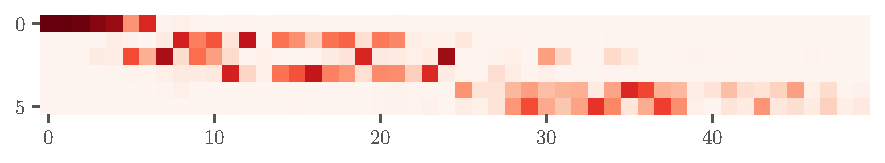
\includegraphics[width=0.45\textwidth]{Figures/Correspondence/LeNet5_fixlr0.01/Conv/xxT_Trueest_real_corr_expand_t50_CIFAR10_Exp1_LeNet5_fixlr0.01_E-1_conv1.pdf}}
%     \subfigure[\small{Correspondence with $\E[\mM].$}]{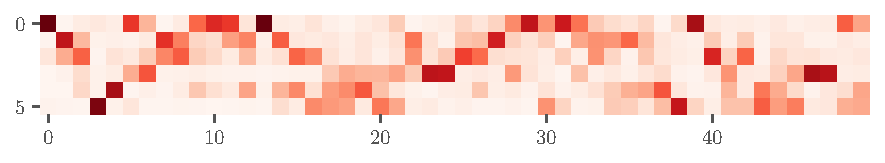
\includegraphics[width=0.45\textwidth]{Figures/Correspondence/LeNet5_fixlr0.01/Conv/UTAU_Trueest_real_corr_expand_t50_CIFAR10_Exp1_LeNet5_fixlr0.01_E-1_conv1.pdf}}
%     \caption{Eigenvector Correspondence for conv1:LeNet5. ($m$=6)}
%     \label{fig:Corr_conv1}
%     \vspace{-1em}
%     % \vspace{-4em}
% \end{figure}

% \begin{figure}[H]
%     \centering
%     \subfigure[\small{Correspondence with $\E[\vx\vx^\T].$}]{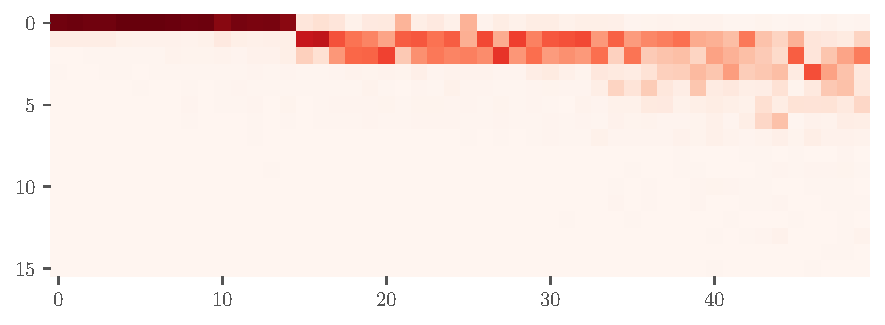
\includegraphics[width=0.45\textwidth]{Figures/Correspondence/LeNet5_fixlr0.01/Conv/xxT_Trueest_real_corr_expand_t50_CIFAR10_Exp1_LeNet5_fixlr0.01_E-1_conv2.pdf}}
%     \subfigure[\small{Correspondence with $\E[\mM].$}]{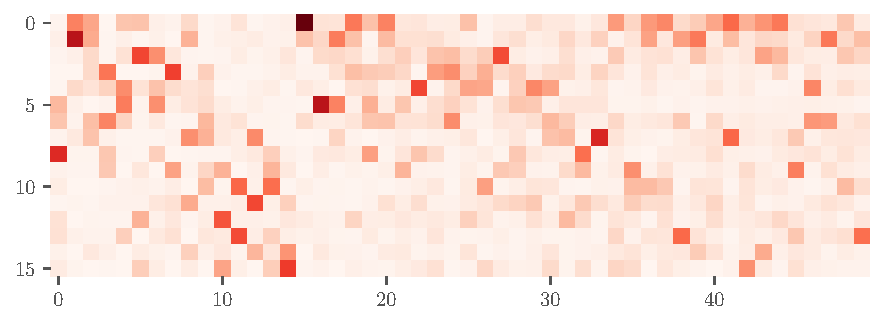
\includegraphics[width=0.45\textwidth]{Figures/Correspondence/LeNet5_fixlr0.01/Conv/UTAU_Trueest_real_corr_expand_t50_CIFAR10_Exp1_LeNet5_fixlr0.01_E-1_conv2.pdf}}
%     \caption{Eigenvector Correspondence for conv2:LeNet5. ($m$=16)}
%     \label{fig:Corr_conv2}
%     \vspace{-1em}
%     % \vspace{-4em}
% \end{figure}

For VGG11 we also observe a strong correlation with the first eigenvector of $\E[\vx\vx^\T]$.

% \begin{figure}[H]
%     \centering
%     % \captionsetup{justification=centering}
%     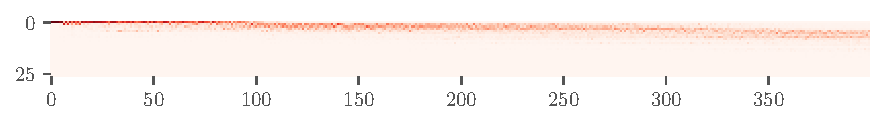
\includegraphics[width=0.8\textwidth]{Appendix_Figures/Correspondance/xxT_Truexxt_corr_expand_t400_CIFAR10_Exp1_VGG11_nobn_fixlr0.01_E-1_features.0.pdf}
%     \caption{Eigenvector Correspondence with $\E[\vx\vx^\T]$ for conv1:VGG11. ($m$=64)}
%     \label{fig:Corr_VGG_conv1}
% \end{figure}

% \begin{figure}[H]
%     \centering
%     % \captionsetup{justification=centering}
%     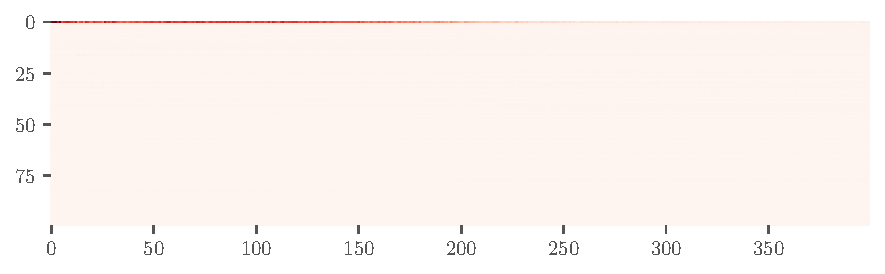
\includegraphics[width=0.8\textwidth]{Appendix_Figures/Correspondance/xxT_Truexxt_corr_expand_t400_CIFAR10_Exp1_VGG11_nobn_fixlr0.01_E-1_features.3.pdf}
%     \caption{Eigenvector Correspondence with $\E[\vx\vx^\T]$ for conv2:VGG11. ($m$=128)}
%     \label{fig:Corr_VGG_conv2}
% \end{figure}
% \begin{figure}[th]
%     \centering
%     \subfigure[\small{Correspondence with $\E[\vx\vx^\T].$}]{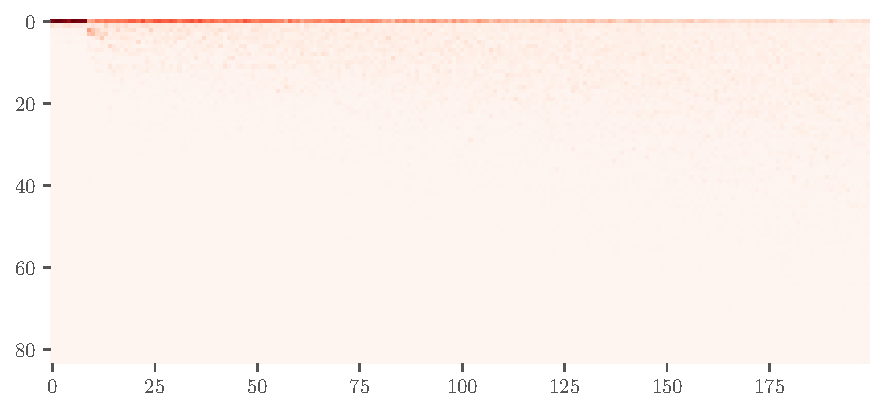
\includegraphics[width=0.45\textwidth]{Figures/Correspondence/LeNet5_fixlr0.01/xxT_Trueest_real_corr_expand_t200_CIFAR10_Exp1_LeNet5_fixlr0.01R2_E-1_fc2.pdf}}
%     \subfigure[\small{Correspondence with $\E[\mM].$}]{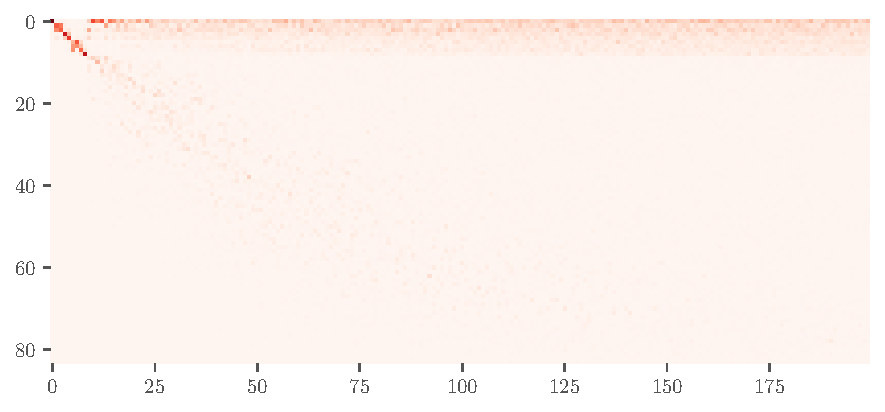
\includegraphics[width=0.45\textwidth]{Figures/Correspondence/LeNet5_fixlr0.01/UTAU_Trueest_real_corr_expand_t200_CIFAR10_Exp1_LeNet5_fixlr0.01R2_E-1_fc2.pdf}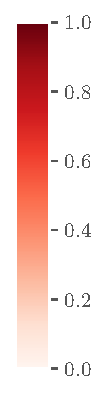
\includegraphics[width=0.06\textwidth]{Figures/Misc/colorbar.pdf}}
%     \caption{Eigenvector Correspondence for fc2:LeNet5. ($m$=84)}
%     \label{fig:Corr_fc2}
%     \vspace{-1em}
%     % \vspace{-4em}
% \end{figure}


% \begin{figure}[H]
%     \centering
%     \begin{subfigure}[t]{0.5\textwidth}
%         \centering
%         \captionsetup{justification=centering}
%         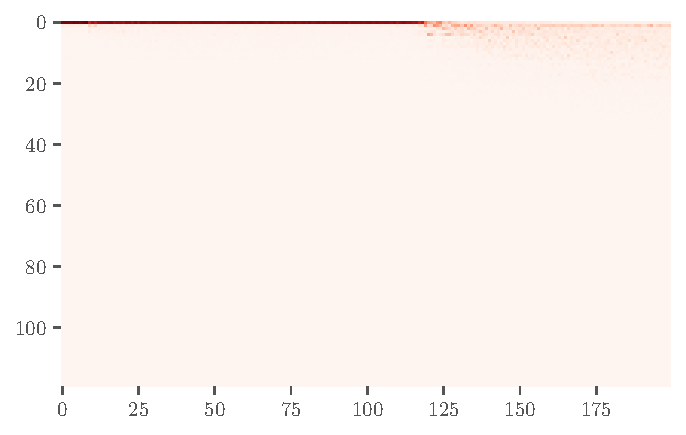
\includegraphics[width=\textwidth]{Figures/Correspondence/LeNet5_fixlr0.01/xxT_Trueest_real_corr_expand_t200_CIFAR10_Exp1_LeNet5_fixlr0.01R2_E-1_fc1.pdf}
%         \caption{Correspondence with $\E[\vx\vx^\T].$}
%         \label{fig:Corr_xxT_True_fc1}
%     \end{subfigure}%
%     \begin{subfigure}[t]{0.5\textwidth}
%         \centering
%         \captionsetup{justification=centering}
%         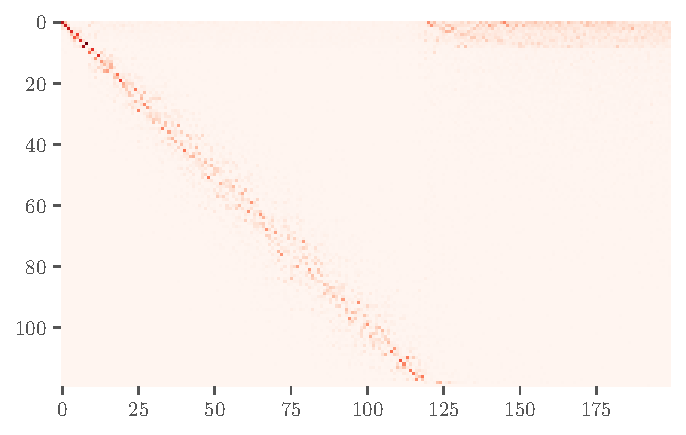
\includegraphics[width=\textwidth]{Figures/Correspondence/LeNet5_fixlr0.01/UTAU_Trueest_real_corr_expand_t200_CIFAR10_Exp1_LeNet5_fixlr0.01R2_E-1_fc1.pdf}
%         \caption{Correspondence with $\E[\mM].$}
%         \label{fig:Corr_UTAU_True_fc1}
%     \end{subfigure}
%     \caption{Eigenvector Correspondence for fc1:LeNet5. ($m$=120)}
%     \label{fig:Corrfc11}
% \end{figure}

% \begin{figure}[H]
%     \centering
%     \begin{subfigure}[t]{0.5\textwidth}
%         \centering
%         \captionsetup{justification=centering}
%         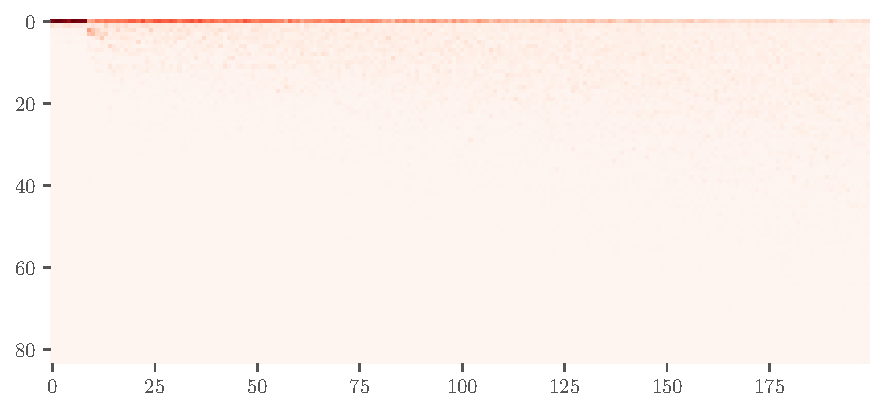
\includegraphics[width=\textwidth]{Figures/Correspondence/LeNet5_fixlr0.01/xxT_Trueest_real_corr_expand_t200_CIFAR10_Exp1_LeNet5_fixlr0.01R2_E-1_fc2.pdf}
%         \caption{Correspondence with $\E[\vx\vx^\T].$}
%         \label{fig:Corr_xxT_True_fc2}
%     \end{subfigure}%
%     \begin{subfigure}[t]{0.5\textwidth}
%         \centering
%         \captionsetup{justification=centering}
%         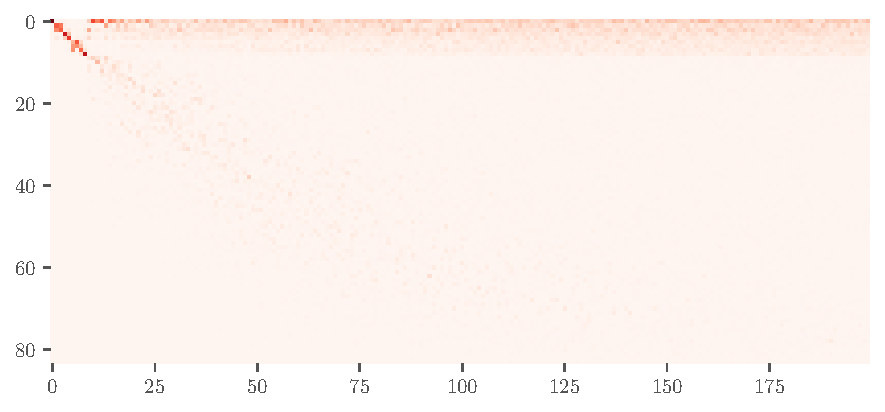
\includegraphics[width=\textwidth]{Figures/Correspondence/LeNet5_fixlr0.01/UTAU_Trueest_real_corr_expand_t200_CIFAR10_Exp1_LeNet5_fixlr0.01R2_E-1_fc2.pdf}
%         \caption{Correspondence with $\E[\mM].$}
%         \label{fig:Corr_UTAU_True_fc2}
%     \end{subfigure}
%     \caption{Eigenvector Correspondence for fc2:LeNet5. ($m$=84)}
%     \label{fig:Corrfc11}
% \end{figure}

% \begin{figure}[H]
%     \centering
%     \begin{subfigure}[t]{0.5\textwidth}
%         \centering
%         \captionsetup{justification=centering}
%         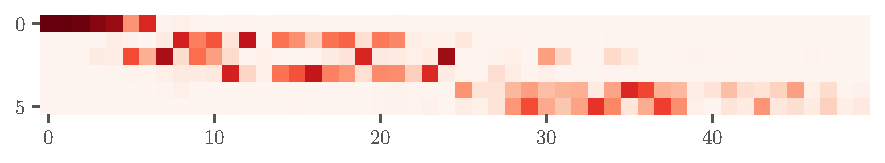
\includegraphics[width=\textwidth]{Figures/Correspondence/LeNet5_fixlr0.01/Conv/xxT_Trueest_real_corr_expand_t50_CIFAR10_Exp1_LeNet5_fixlr0.01_E-1_conv1.pdf}
%         \caption{Correspondence with $\E[\vx\vx^\T].$}
%         \label{fig:Corr_xxT_True_conv1}
%     \end{subfigure}%
%     \begin{subfigure}[t]{0.5\textwidth}
%         \centering
%         \captionsetup{justification=centering}
%         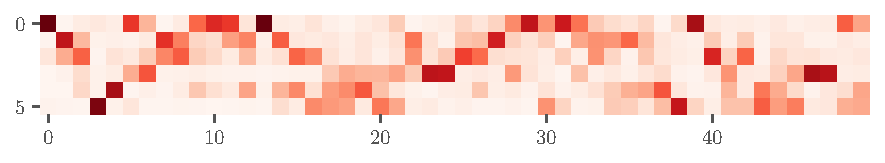
\includegraphics[width=\textwidth]{Figures/Correspondence/LeNet5_fixlr0.01/Conv/UTAU_Trueest_real_corr_expand_t50_CIFAR10_Exp1_LeNet5_fixlr0.01_E-1_conv1.pdf}
%         \caption{Correspondence with $\E[\mM].$}
%         \label{fig:Corr_UTAU_True_conv1}
%     \end{subfigure}
%     \caption{Eigenvector Correspondence for conv1:LeNet5. ($m$=6)}
%     \label{fig:Corr_conv1}
% \end{figure}

% \begin{figure}[H]
%     \centering
%     \begin{subfigure}[t]{0.5\textwidth}
%         \centering
%         \captionsetup{justification=centering}
%         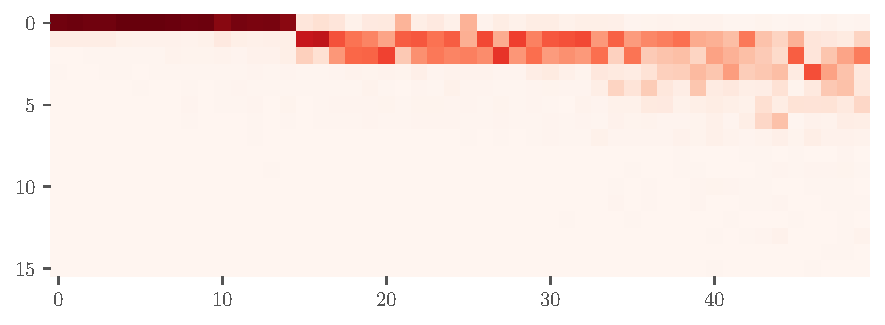
\includegraphics[width=\textwidth]{Figures/Correspondence/LeNet5_fixlr0.01/Conv/xxT_Trueest_real_corr_expand_t50_CIFAR10_Exp1_LeNet5_fixlr0.01_E-1_conv2.pdf}
%         \caption{Correspondence with $\E[\vx\vx^\T].$}
%         \label{fig:Corr_xxT_True_conv2}
%     \end{subfigure}%
%     \begin{subfigure}[t]{0.5\textwidth}
%         \centering
%         \captionsetup{justification=centering}
%         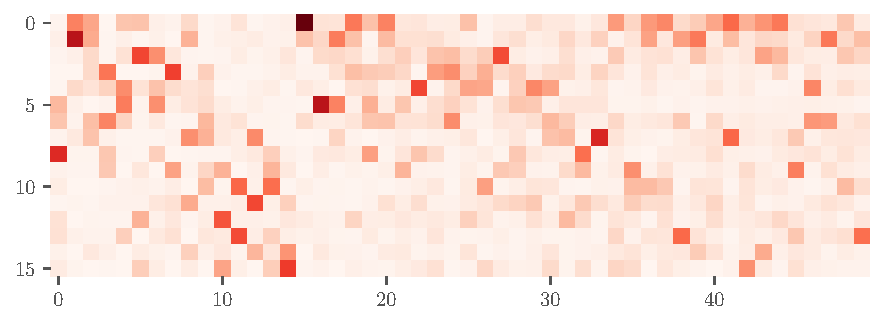
\includegraphics[width=\textwidth]{Figures/Correspondence/LeNet5_fixlr0.01/Conv/UTAU_Trueest_real_corr_expand_t50_CIFAR10_Exp1_LeNet5_fixlr0.01_E-1_conv2.pdf}
%         \caption{Correspondence with $\E[\mM].$}
%         \label{fig:Corr_UTAU_True_conv2}
%     \end{subfigure}
%     \caption{Eigenvector Correspondence for conv2:LeNet5. ($m$=16)}
%     \label{fig:Corr_conv2}
% \end{figure}

% For VGG11 we also observe a strong correlation with the first eigenvector of $\E[\vx\vx^\T]$. However the phenomenon is not as strong as the ones exhibited by LeNet5.

\begin{figure}[H]
    \centering
    \captionsetup{justification=centering}
    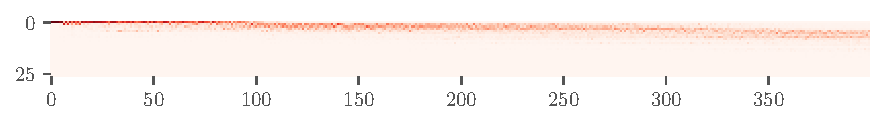
\includegraphics[width=0.8\textwidth]{Appendix_Figures/Correspondance/xxT_Truexxt_corr_expand_t400_CIFAR10_Exp1_VGG11_nobn_fixlr0.01_E-1_features.0.pdf}

    \caption{Eigenvector Correspondence with $\E[\vx\vx^\T]$ for conv1:VGG11. ($m$=64)}
    \label{fig:Corr_VGG_conv1}
\end{figure}

\begin{figure}[H]
    \centering
    \captionsetup{justification=centering}
    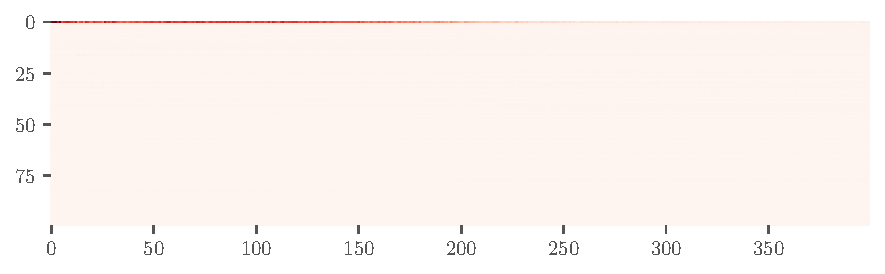
\includegraphics[width=0.8\textwidth]{Appendix_Figures/Correspondance/xxT_Truexxt_corr_expand_t400_CIFAR10_Exp1_VGG11_nobn_fixlr0.01_E-1_features.3.pdf}

    \caption{Eigenvector Correspondence with $\E[\vx\vx^\T]$ for conv2:VGG11. ($m$=128)}
    \label{fig:Corr_VGG_conv2}
\end{figure}

\begin{figure}[H]
    \centering
    \captionsetup{justification=centering}
    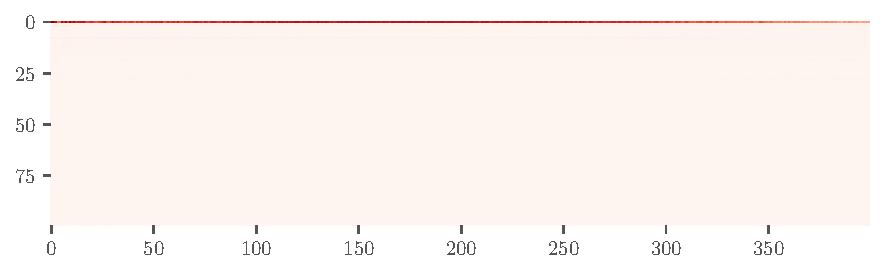
\includegraphics[width=0.8\textwidth]{Appendix_Figures/Correspondance/xxT_Truexxt_corr_expand_t400_CIFAR10_Exp1_VGG11_nobn_fixlr0.01_E-1_features.6.pdf}

    \caption{Eigenvector Correspondence with $\E[\vx\vx^\T]$ for conv3:VGG11. ($m$=256)}
    \label{fig:Corr_VGG_conv2}
\end{figure}